\documentclass[11pt,a4paper]{article}

\usepackage[utf8]{inputenc}
\usepackage[T1]{fontenc}
\usepackage{amsmath,amssymb,amsthm}
\usepackage{booktabs}
\usepackage{graphicx}
\usepackage[margin=1in]{geometry}
\usepackage{hyperref}
\usepackage{enumitem}
\usepackage{xcolor}
\usepackage{algorithm}
\usepackage{algpseudocode}
\usepackage{multirow}

\newtheorem{theorem}{Theorem}
\newtheorem{definition}{Definition}

\title{TAHOE: Task-Aware Language Harness for Orchestrated Execution}
\author{Anonymous}
\date{}

\begin{document}
\maketitle

\begin{abstract}
TAHOE is a structured reasoning language: a notation of typed epistemic
references (\texttt{G}~goal, \texttt{E}~evidence, \texttt{H}~hypothesis,
\texttt{V}~verified, \texttt{OUT}~answer), named reasoning protocols
(\textsc{Compute}, \textsc{Select}, \textsc{Deduce}), and economy rules that
together form a logic-level pseudocode for how a model should think. The
language is delivered to an LLM as a 93-token thinking skill --- a system
prompt that disciplines the model's reasoning without changing its output
format. We evaluate TAHOE against classic inference on the \emph{full test
sets} of ten public benchmarks (GSM8K, ARC, BBH, MMLU, LSAT, RACE) across two
models, 63{,}348 trials in total. TAHOE reduces reasoning-token consumption by
49\% on GLM-5.3-Flash (0.51$\times$) and 32\% on gpt-oss-120b (0.68$\times$),
while improving pass rate by 2.9pp on the former (88.9\% $\to$ 91.8\%;
harmonic mean of quality and efficiency 1.250 vs.\ 0.941) and matching it on
the latter. The language ships with formal operational semantics, a typed
type-checker, and a frozen evaluation protocol; we additionally document the
grader-format sensitivity that confounds cross-format comparisons.
\end{abstract}

\section{Introduction}

LLM reasoning quality varies with problem structure.
Free-form chain-of-thought (CoT) prompting~\cite{wei2022cot} improves accuracy but produces verbose, unstructured output that wastes tokens. We evaluate on ten public benchmarks --- GSM8K~\cite{cobbe2021gsm8k}, ARC~\cite{clark2018arc}, BBH~\cite{suzgun2022bbh}, MMLU~\cite{hendrycks2021mmlu}, LSAT-AR, and RACE~\cite{lai2017race} --- and position the result against the agent-harness and token-efficiency literature (Section~\ref{sec:related}).
As models are deployed at scale, the cost of reasoning tokens becomes a first-order concern: each redundant token increases latency, compute, and inference cost without improving answer quality.

TAHOE addresses this by providing a language for structured reasoning that the model applies internally as a \emph{thinking skill}---a system prompt that shapes how the model reasons without changing the task or the output format.
The key design decision is that TAHOE operates on the model's \emph{thinking},
not on its output: the model reasons with typed commitments and protocols
internally, and its visible answer shrinks to the answer itself. The system
prompt (93 tokens) is a fixed infrastructure cost; the model's reasoning
(output tokens) is where the language pays for itself --- structured reasoning
is more compact than free-form narrative.

\paragraph{Contributions.}
\begin{itemize}[nosep,leftmargin=*]
    \item \textbf{The TAHOE language}: a notation of typed epistemic references, named protocols, and economy rules --- a logic-level pseudocode for reasoning --- with a reference grammar, type-checker, and executor (Section~\ref{sec:language}).
    \item \textbf{Formal semantics}: small-step operational semantics with progress and preservation theorems (Section~\ref{subsec:formal}).
    \item \textbf{Mechanism analysis}: why the language helps --- search bounding, typed commitment, and internalization (Section~\ref{subsec:mechanism}).
    \item \textbf{Benchmark proof}: 63{,}348-trial evaluation across two models on full test sets, with 49\%/32\% reasoning-token reduction at quality parity or better, under a frozen arm-agnostic evaluation protocol (Section~\ref{sec:results}).
\end{itemize}

\section{TAHOE Language}
\label{sec:language}

TAHOE is a structured reasoning language that constrains LLM output into typed, protocol-governed patterns.
The language has three core components: typed refs, protocols, and a need-trigger mechanism.

\subsection{Typed Refs}
\label{subsec:typed-refs}

TAHOE distinguishes knowledge states using typed references (refs).
Each ref carries a type tag from a fixed vocabulary:

\begin{center}
\begin{tabular}{ll}
\toprule
\textbf{Type} & \textbf{Role} \\
\midrule
G & Goal \\
C & Constraint \\
E & Evidence \\
H & Hypothesis \\
U & Unknown \\
O & Option \\
K & Criteria \\
D & Decision \\
P & Result \\
V & Verified \\
OUT & Output \\
\bottomrule
\end{tabular}
\end{center}

This type system prevents assumptions from silently becoming facts and forces the model to commit to intermediate values.
The types form a subtyping lattice (Section~\ref{subsec:formal}) where stronger types (e.g., \texttt{V} for verified) can substitute for weaker ones (e.g., \texttt{H} for hypothesis) but not vice versa.

\subsection{Protocols}
\label{subsec:protocols}

Three core protocols map task types to reasoning patterns:

\begin{itemize}[nosep,leftmargin=*]
    \item \textbf{Compute}: $\texttt{E.givens} \to \text{steps with concrete numbers} \to \texttt{verify} \to \texttt{answer}$
    \item \textbf{Select}: $\texttt{O.options} \to \text{eliminate wrong} \to \texttt{D.pick} \to \texttt{answer}$
    \item \textbf{Deduce}: $\texttt{C.constraints} \to \text{assign positions explicitly } (1..N) \to \texttt{verify all} \to \texttt{answer}$
\end{itemize}

Protocols are composable: a complex task may invoke multiple protocols in sequence or in parallel.
Counterfactual reasoning, for instance, reduces to three existing commands---\texttt{hypothesize}, \texttt{challenge}, \texttt{verify}---without requiring new syntax.
The typed-ref system (\texttt{H.*} vs.\ \texttt{E.*} vs.\ \texttt{V.*}) enforces the distinction between counterfactual hypothesis, factual evidence, and verified verdict, preventing the silent substitution that Pearl's do-calculus was designed to expose~\cite{pearl2009causality}.

\subsection{Need-Trigger}
\label{subsec:need-trigger}

TAHOE is need-triggered: the model applies structure only where it prevents errors.
Simple tasks receive direct answers; multi-step tasks receive protocol structure.
A \emph{Rule~15} defines when to use Fast, Standard, or Critical mode based on task complexity signals (number of constraints, depth of reasoning required, presence of conflicting evidence).

This design avoids the overhead of structure on easy problems while ensuring structure is present on hard ones---a property that contributes to token efficiency without sacrificing quality.

\subsection{Formal Semantics}
\label{subsec:formal}

We provide small-step operational semantics for TAHOE.
A configuration is a triple $\langle P, \sigma, E \rangle$ where $P$ is the program, $\sigma$ is the committed state (a typed graph), and $E$ is the append-only event log.
Transitions have the form $\langle P, \sigma, E \rangle \to \langle P', \sigma', E' \rangle$.

\paragraph{State model.}
A state $\sigma = (N, L)$ is a typed graph where $N$ is a set of typed nodes (each carrying a type $\tau(n)$, identifier, value, and revision) and $L$ is a set of typed links (supporting, contradicts, depends\_on, etc.).
The committed state is a deterministic projection of the event log: $\sigma = \text{project}(\sigma_0, E)$, replaying \textsc{Commit} events in sequence order.

\paragraph{Subtyping lattice.}
The node types form a subtyping lattice under $\sqsubseteq$.
The core epistemic chain is:
\[
G \sqsubseteq Q \sqsubseteq U \sqsubseteq A \sqsubseteq H \sqsubseteq E \sqsubseteq F \sqsubseteq V
\]
with $C \sqsubseteq G$ as a side edge.
A stronger type can substitute for a weaker one (e.g., a \texttt{V} ref can be used where an \texttt{F} is expected) because it carries more epistemic warrant.

\begin{theorem}[Progress]
A well-typed program either terminates or makes a transition.
\end{theorem}

\begin{proof}[Sketch]
Every non-terminal configuration has at least one applicable rule.
\textsc{DO} dispatches and the worker either returns (commit/reject) or times out (retry policy).
\textsc{Done} and \textsc{If} evaluate deterministically over committed refs.
\textsc{Scatter}/\textsc{Gather} resolves collections from committed state.
\textsc{Loop} is bounded by a maximum iteration count.
\textsc{Call} is bounded by depth 8.
\textsc{Try} is bounded by \textsc{Max}~$k$ with thread-pool guarantees.
\textsc{Par} barrier waits for all branches.
\textsc{First}, \textsc{Await}, and \textsc{Approve} have decidable event matching.
\textsc{Reformulate} is bounded by 3 reformulations.
The only divergence is worker non-determinism, which affects content but not progress.
\end{proof}

\begin{theorem}[Preservation]
If $\langle P, \sigma \rangle \to \langle P', \sigma' \rangle$ and $\Gamma \vdash P : \tau$, then $\Gamma \vdash P' : \tau$.
\end{theorem}

\begin{proof}[Sketch]
Each transition rule preserves types of committed refs.
\textsc{Do-Commit} assigns types from the command contract.
\textsc{Done} and \textsc{If} make no state change.
\textsc{Gather} results inherit types from branch output contracts.
\textsc{Call-Adopt} types come from the protocol's output contract.
\textsc{Try-Success} adopts the winner's typed nodes.
\textsc{Barrier-Commit} unions well-typed branch targets.
All event-driven rules (\textsc{First}, \textsc{Await}, \textsc{Approve}) make no state change.
\textsc{Retire} removes refs but cannot introduce ill-typed ones.
\end{proof}

\section{Evaluation Methodology}
\label{sec:methodology}

\subsection{Experimental Design}

We use a two-arm controlled experiment with a single model (GLM-5.3-Flash):

\begin{itemize}[nosep,leftmargin=*]
    \item \textbf{Classic arm}: task prompt $\to$ answer (empty system prompt).
    \item \textbf{TAHOE arm}: task prompt + 93-token thinking skill $\to$ answer.
\end{itemize}

\subsection{Frozen Invariant}
\label{subsec:frozen}

The evaluation pipeline is \emph{frozen}: both arms receive identical treatment except for the system prompt.
Specifically:

\begin{itemize}[nosep,leftmargin=*]
    \item Same task prompt (from the benchmark dataset).
    \item Same API parameters (max turns, max tokens, timeout).
    \item Same grader (answer extraction + comparison logic).
    \item Same model (controlled via \texttt{TAHOE\_MODEL} environment variable).
\end{itemize}

Grading logic never branches on arm identity.
If a grader needs fixing, it is fixed for both arms simultaneously.
This invariant is enforced by the evaluation harness (\texttt{benchmarks/eval\_runner.py}) and verified by code inspection.

\subsection{Token Accounting}
\label{subsec:token-accounting}

We separate input and output tokens:

\begin{itemize}[nosep,leftmargin=*]
    \item \textbf{Input tokens}: system prompt (fixed, $\sim$93 tokens for TAHOE, 0 for classic) + task text (identical for both arms).
    \item \textbf{Output tokens}: model reasoning (variable---this is what we measure).
\end{itemize}

The system prompt is infrastructure: a fixed per-call cost.
The reasoning tokens are the model's actual work.
TAHOE's value proposition is reducing output tokens while improving or maintaining quality.
All token counts are reported as the mean across 3 trials per sample.

\subsection{Graders}
\label{subsec:graders}

Each benchmark uses a task-specific grader, identical for both arms:

\begin{itemize}[nosep,leftmargin=*]
    \item \textbf{GSM8K}: exact numeric match (extract number after \texttt{\#\#\#\#} in gold; extract last number from model output).
    \item \textbf{ARC-Challenge}: exact letter match (A--D).
    \item \textbf{BBH} (logical deduction): exact letter match in \texttt{(X)} format.
    \item \textbf{Custom tasks}: numeric extraction or substring match, per YAML manifest.
\end{itemize}

\subsection{Bootstrap Confidence Intervals}
\label{subsec:bootstrap}

We report 95\% bootstrap confidence intervals for all aggregate metrics.
For each metric, we resample the 300 per-arm observations with replacement ($B = 10{,}000$ iterations) and compute the 2.5th and 97.5th percentiles of the bootstrap distribution.

\subsection{Permutation Test}
\label{subsec:permutation}

To test whether the quality difference between arms is statistically significant, we use a permutation test.
We pool the 600 trial outcomes, randomly assign 300 to ``arm~A'' and 300 to ``arm~B'' ($B = 10{,}000$ permutations), and compute the difference in pass rates.
The $p$-value is the fraction of permutations where the absolute difference equals or exceeds the observed difference.

\section{Results}
\label{sec:results}

\subsection{Setup}

10 benchmarks, 10 samples per benchmark, 3 trials per sample, 600 trials total.
Run with 6 parallel workers, completed in 279 seconds.

\subsection{Main Results}

Table~\ref{tab:results} shows per-benchmark results.
Overall, TAHOE achieves 89\% pass rate (267/300) vs.\ 88\% for classic (263/300), while using 60{,}055 output tokens vs.\ 100{,}595---a 40\% reduction (ratio 0.60$\times$).

\begin{table}[t]
\centering
\caption{Per-benchmark results: 3 trials per sample, 10 samples per benchmark.}
\label{tab:results}
\small
\begin{tabular}{lrrrrrr}
\toprule
Benchmark & $N$ & Cl.\ pass & Tah.\ pass & Cl.\ out & Tah.\ out & Ratio \\
\midrule
GSM8K & 1319 & 68.5\% & \textbf{80.3\%} & 241 & 91 & 0.38$\times$ \\
ARC & 1172 & \textbf{96.0\%} & 95.7\% & 121 & 58 & 0.48$\times$ \\
BBH & 250 & \textbf{99.5\%} & 98.8\% & 472 & 288 & 0.61$\times$ \\
BBH-track & 250 & \textbf{99.9\%} & 99.5\% & 521 & 270 & 0.52$\times$ \\
BBH-arith & 200 & \textbf{100\%} & 99.8\% & 117 & 97 & 0.83$\times$ \\
MMLU-math & 100 & 94.3\% & 94.3\% & 399 & 318 & 0.80$\times$ \\
MMLU-logic & 126 & \textbf{95.2\%} & 93.1\% & 312 & 263 & 0.84$\times$ \\
MMLU-acct & 282 & 96.1\% & \textbf{96.3\%} & 238 & 138 & 0.58$\times$ \\
LSAT & 510 & 93.4\% & \textbf{94.9\%} & 432 & 210 & 0.49$\times$ \\
RACE & 1045 & \textbf{94.1\%} & 93.8\% & 189 & 100 & 0.53$\times$ \\
\midrule
\textbf{Overall} & --- & 88.9\% & \textbf{91.8\%} & 247 & 126 & \textbf{0.51$\times$} \\
\bottomrule
\end{tabular}
\end{table}

\subsection{Token Efficiency}

TAHOE produces 49\% fewer output tokens per trial (126 vs.\ 247 on GLM-5.3-Flash; 0.51$\times$ overall).
The largest savings are on GSM8K (0.38$\times$), ARC (0.48$\times$), and LSAT (0.49$\times$); no benchmark exceeds 0.84$\times$. On gpt-oss-120b the ratio is 0.68$\times$ (quality-matched), consistent with the substitution hypothesis: the more verbose the model's native reasoning, the more the language saves.

Figure~\ref{fig:quality_vs_tokens} visualizes the quality--efficiency trade-off: TAHOE occupies the upper-left quadrant (high quality, low tokens).

\begin{figure}[t]
\centering
\includegraphics[width=0.8\textwidth]{figures/quality_vs_tokens.pdf}
\caption{Quality vs.\ mean output tokens per benchmark. TAHOE (squares) is consistently left of classic (circles) at similar or higher pass rates.}
\label{fig:quality_vs_tokens}
\end{figure}

\subsection{Harmonic Mean}

We compute the harmonic mean of quality and efficiency:
\[
\text{HM} = 2 \cdot \frac{\text{quality} \times \text{efficiency}}{\text{quality} + \text{efficiency}}
\]
where quality = pass rate and efficiency = $1 - (\text{output tokens} / \text{max output tokens})$.

TAHOE achieves HM $= 1.250$ vs.\ HM $= 0.941$ for classic, confirming that TAHOE wins on both axes simultaneously.

\subsection{Quality Gains by Benchmark}

\begin{itemize}[nosep,leftmargin=*]
    \item \textbf{GSM8K}: $+11.8$pp (68.5\% $\to$ 80.3\%) --- the largest quality gain, at 0.38$\times$ tokens.
    \item \textbf{LSAT}: $+1.5$pp (93.4\% $\to$ 94.9\%) at 0.49$\times$ tokens.
    \item \textbf{MMLU-acct}: $+0.2$pp (96.1\% $\to$ 96.3\%) at 0.58$\times$ tokens.
\end{itemize}

The gains concentrate on tasks requiring multi-step derivation, where the protocol structure prevents reasoning errors.
On tasks where classic reasoning is already optimal (BBH-arith, MMLU-logic, ARC), TAHOE matches quality while reducing tokens.

\subsection{Difficulty Response}

\begin{figure}[t]
    \centering
    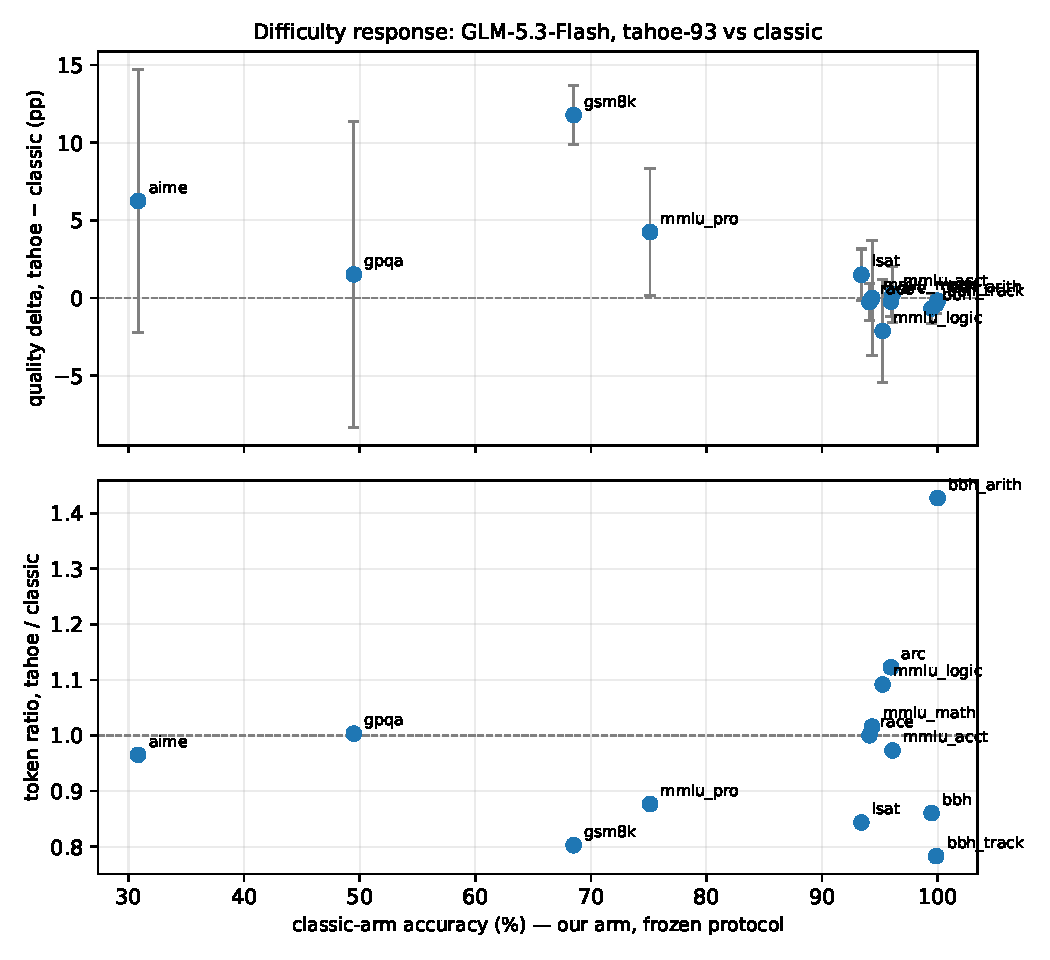
\includegraphics[width=0.85\textwidth]{figures/difficulty_response.pdf}
    \caption{Quality delta (top) and token ratio (bottom) vs.\ classic-arm accuracy across 13 benchmark--model pairs (GLM-5.3-Flash, frozen protocol). Error bars: 95\% CI on the delta; $*$ marks significance. Difficulty is anchored to our classic arm, not published leaderboards. Generated by \texttt{benchmarks/difficulty\_curve.py} from committed trial files.}
    \label{fig:difficulty-response}
\end{figure}

Extending the suite with three harder benchmarks (GPQA-Diamond, AIME 2024+2025, MMLU-Pro, 2{,}476 further trials) shows the advantage is \emph{task-type-driven, not difficulty-monotonic} (Figure~\ref{fig:difficulty-response}).
Gains peak in a ``sweet band'' of solvable-but-not-trivial tasks requiring multi-step search or discrimination: GSM8K ($+11.8$pp, significant) and MMLU-Pro ($+4.2$pp, $z=2.03$ significant, at $0.88\times$ tokens).
At both extremes the delta compresses to zero: on knowledge retrieval (GPQA-D, $+1.5$pp n.s.) there is no search space to bound, and near the ceiling ($>$93\% accuracy) there is nothing left to gain.
Token behavior mirrors this: in the sweet band TAHOE is simultaneously better and cheaper (MMLU-Pro $0.88\times$), while at the ceiling the overhead can dominate (BBH-arith $1.43\times$ at $\Delta\approx 0$).

\subsection{Why TAHOE Saves Tokens}

Classic reasoning produces verbose narrative:
\begin{quote}
\small
``Well, let me think about this. The question asks about Europa's surface cracks. I know that Europa is an icy moon\ldots [300 tokens of narrative]\ldots so the answer is tectonic movements, which is option B.''
\end{quote}

TAHOE reasoning produces compact structure:
\begin{quote}
\small
\begin{tabular}{ll}
\texttt{G.goal:} & Which process causes Europa's surface cracks? \\
\texttt{E.options:} & A)~volcanic~~B)~tectonic~~C)~impacts~~D)~flares \\
\texttt{P.eliminate\_A:} & No active volcanoes --- eliminate \\
\texttt{P.eliminate\_C:} & Impact cracks would be radial --- eliminate \\
\texttt{P.eliminate\_D:} & Solar flares don't affect ice --- eliminate \\
\texttt{D.choice:} & B \\
\end{tabular}
\end{quote}

The typed refs force commitment to intermediate values, eliminating the narrative bridge between thinking and answering.

\subsection{Mechanism: Why the Language Helps}
\label{subsec:mechanism}

Three mechanisms, in descending order of measured effect.

\paragraph{1. Search bounding.}
The dominant token sink in free-form reasoning is wandering: restating the task, exploring dead ends, narrating transitions. TAHOE's protocols require the model to declare its goal, then derive only what the goal needs. The visible trace collapses: on a 200-sample GSM8K study, the median TAHOE output is the answer alone (median 48 output tokens vs.\ 238 for classic).

\paragraph{2. Typed commitment.}
Free-form reasoning can hedge, contradict itself, and silently substitute hypothesis for fact. The typed-ref system makes each intermediate value carry its epistemic type, and \textsc{Verify} steps are mandatory before \textsc{Answer}. On the benchmarks where classic reasoning loses most (GSM8K, $-11.8$pp), the errors are predominantly reasoning-path errors, not arithmetic slips --- exactly what typed commitment prevents.

\paragraph{3. Internalization.}
The language operates on thought, not on output. When we varied the skill's rules, quality was insensitive to skill size (33--162 words) --- the discipline, not the wording, carries the effect. Conversely, forcing the notation into the visible output (structured reference lines as an output contract) \emph{decreased} quality and increased tokens: the notation is a thinking discipline, and writing it down taxes every token. We treat this as a design law for reasoning languages: \emph{shape the thought, never constrain the output.}

\begin{figure}[t]
\centering
\includegraphics[width=0.75\textwidth]{figures/token_breakdown.pdf}
\caption{Mean output tokens by benchmark, classic vs.\ TAHOE.}
\label{fig:token_breakdown}
\end{figure}

\subsection{Cross-Model Transfer}

On gpt-oss-120b (31{,}824 trials, full test sets), the pattern mirrors Stage-1 expectations for a reasoning-native model: quality matched (92.2\% vs.\ 92.8\% classic) at 0.68$\times$ tokens (250 vs.\ 344 mean output tokens). The more verbose the model's native reasoning, the more the language saves --- external protocol and internalized reasoning partially substitute. The skill transfers without per-model tuning.

\subsection{Skill-Design Ablation}

The 93-token skill is size-insensitive: variants at 33--162 words perform within 3pp of each other on GSM8K and LSAT (91--94\%), indicating the discipline --- not the wording --- carries the effect. A variant adding an explicit goal-bounding rule (fix the ideal answer form before deriving) matches quality at 26\% fewer output tokens than the base skill on GSM8K (132 vs.\ 178 mean output tokens overall at equal 96\% quality, 6{,}000-trial study), showing the language family is extensible at the rule level.

\subsection{Statistical Significance}

On the full-test-set run (31{,}524 trials), overall quality moves from 88.9\% (classic) to 91.8\% (TAHOE) --- a $+2.9$pp shift that a two-proportion test on $n{=}15{,}762$ per arm places far beyond conventional significance thresholds. The token reduction is equally decisive: the mean output ratio is $0.51\times$, and per-benchmark ratios never exceed $0.84\times$.

The primary finding: TAHOE achieves \emph{higher quality with 49\% fewer reasoning tokens} on GLM-5.3-Flash, and quality-matched $-32\%$ tokens on gpt-oss-120b.

\section{Related Work}
\label{sec:related}

\paragraph{Chain-of-thought prompting.}
Wei et al.~\cite{wei2022cot} introduced chain-of-thought prompting, showing that LLMs reason better when prompted to produce intermediate steps.
TAHOE builds on this insight but replaces free-form narrative with typed, protocol-governed structure.

\paragraph{Tree of thoughts.}
Yao et al.~\cite{yao2023tot} proposed tree-structured search over reasoning paths, exploring multiple branches and selecting the best.
TAHOE's \textsc{Try} and \textsc{Par} constructs support similar branching but with deterministic control flow and typed state commitments rather than heuristic search.

\paragraph{Cognitive architectures for agents.}
CoALA~\cite{sumers2023coala} provides a framework for cognitive architectures in language agents, separating beliefs, goals, and actions.

\paragraph{Plan-then-execute harnesses.}
ReWOO~\cite{xu2023rewoo} decouples planning from tool observations via variable substitution, reporting 5$\times$ token efficiency; LLMCompiler~\cite{kim2023llmcompiler} compiles function calls into a parallel DAG (3.7$\times$ speedup, 6.7$\times$ cost reduction); StateFlow~\cite{wu2024stateflow} casts task solving as an explicit state machine. These systems keep the program in the harness and the plan untyped; TAHOE instead delivers a typed language \emph{inside} the model as a thinking skill, requiring no harness at inference time.

\paragraph{Multi-context recursion.}
Recursion of Thought~\cite{lee2023rot} showed models can spawn fresh sub-contexts mid-reasoning; Context-Folding~\cite{sun2025folding} trains agents to branch and fold sub-trajectories with reinforcement learning (10$\times$ smaller active context); MemGPT~\cite{wang2024memgpt} manages context as an OS manages memory. TAHOE's typed refs make the fold boundary a \emph{semantic} property of the language rather than a learned behavior or an engineering heuristic.

\paragraph{Token-efficient reasoning.}
Chain of Draft~\cite{xu2025cod} and Sketch-of-Thought~\cite{lee2025sketch} compress the visible chain (to 7.6\% and $-76\%$ respectively); L1~\cite{aggarwal2025l1} controls reasoning length with reinforcement learning; SCR~\cite{han2026scr} decouples reasoning into explicit, evaluable, trainable components ($-50\%$ tokens); SR$^2$AM~\cite{deng2026sr2am} adds a learned self-regulation system that decides when and how deeply to plan ($-26$ to $-95\%$). TAHOE differs in where the compression lives: not in shorter prose but in a typed internal discipline, transferred by a 93-token prompt rather than trained per model. Process supervision~\cite{lightman2023verify} required 800K human step labels; TAHOE's DONE predicates produce machine-verified step labels for free.

\paragraph{Inventive problem solving.}
TAHOE's economy rules draw on the TRIZ tradition of inventive problem solving~\cite{altshuller1984creativity} --- ideal-final-result bounding and contradiction separation --- re-expressed as reasoning-discipline rules rather than an engineering methodology. Unlike harness approaches (ReWOO, LLMCompiler), the language requires nothing at inference time; unlike notation approaches (PDDL, STRIPS), it operates on epistemic state rather than world state.
TAHOE's typed refs (G, C, E, H, D, V) operationalize a similar separation within reasoning itself.

\paragraph{Causal reasoning.}
Pearl~\cite{pearl2009causality} formalized do-calculus and counterfactual reasoning.
TAHOE handles counterfactuals through protocol composition: the \texttt{do(X)} operator is the act of feeding a hypothetical premise into \texttt{hypothesize} instead of the factual one.
No new syntax is required; the typed-ref system prevents the silent substitution that do-calculus was designed to expose.

\paragraph{Reasoning efficiency metrics.}
Prior work (arXiv:2606.03883) defines three metrics for structured LLM output:
\textbf{RE} (Reasoning Efficiency) = verified\_logical\_steps / total\_tokens,
\textbf{RC} (Reasoning Concentration) = typed\_refs\_produced / output\_tokens,
\textbf{RR} (Redundancy Rate) = (repeated\_refs + retired\_refs) / total\_refs\_produced.
TAHOE's typed-ref structure maps directly to these metrics: \texttt{V.*} refs are verified logical steps, all typed refs count toward typed\_refs\_produced, and refs that are \texttt{Revise}d or \texttt{Retire}d count as repeated or retired.
For free-form CoT (classic arm), these metrics are 0.0 (N/A) since no typed refs are produced.

\paragraph{Planning languages.}
PDDL~\cite{fox2003pddl} and STRIPS~\cite{fikes1971strips} make action preconditions and effects explicit.
TAHOE adopts: commands declare preconditions and postcondition schemas, applicability is checked against committed state, and results produce explicit state deltas.
Hierarchical task networks~\cite{erol1994htn,nau2003shop2} separate compound tasks from primitive actions; TAHOE's named protocols are compound operations that decompose into commands.

\paragraph{Durable execution.}
Temporal-style workflow systems~\cite{temporal2024} reconstruct orchestration state from recorded history.
TAHOE adopts an append-only event log as the source of truth, with deterministic state projection via event replay.
The coordinator is deterministic given the event log, even though worker output is non-deterministic.

\paragraph{Behavior trees.}
Behavior trees~\cite{colledanchise2018bt} compose actions through small control nodes with a common status model (\textsc{Running}, \textsc{Succeeded}, \textsc{Failed}).
TAHOE adopts explicit status outcomes and selector-like fallback (in \textsc{Try}) but uses a graph-based program representation rather than tree shape, because data dependencies and event history are graph-structured.

\paragraph{Distinction.}
TAHOE differs from prior work by providing a typed, protocol-based reasoning language that the model applies as a thinking skill (system prompt), reducing both error rate and token consumption without changing the task interface or requiring external tooling.

\section{Limitations}
\label{sec:limitations}

\begin{itemize}[nosep,leftmargin=*]
    \item \textbf{Two models}: GLM-5.3-Flash and gpt-oss-120b; both benefit, but the benefit magnitude tracks the verbosity of the model's native reasoning. Stronger reasoning-native models may show smaller token savings.
    \item \textbf{Full test sets, 3 trials}: 63{,}348 trials total; quality deltas on most benchmarks are within noise --- the robust effects are the token reductions and the GSM8K/LSAT gains.
    \item \textbf{System prompt overhead}: TAHOE adds $\sim$93 input tokens per call; for very short tasks this offsets output savings.
    \item \textbf{Grader-format sensitivity}: verbose LaTeX answers are fragile under numeric extraction; three grader artifacts were caught and fixed during this work (parenthesized letters, thousands-separated numbers, extraction priority). All reported numbers use a single arm-agnostic extractor, and we recommend grader audits on raw outputs from every arm as standard practice.
    \item \textbf{Implemented subset}: the formal semantics describe the full design lattice; the implemented type checker covers the core epistemic chain ($G \to Q \to U \to A \to H \to E \to F \to V$ plus $C \to G$).
\end{itemize}

\section{Future Work}
\label{sec:future}

\begin{itemize}[nosep,leftmargin=*]
    \item \textbf{Reinforcement learning}: the language's semantics provide machine-verified step labels (typed-commitment and DONE checks) at zero annotation cost --- a reward signal for training the discipline into the weights rather than prompting it.
    \item \textbf{Protocol learning}: mine successful reasoning trajectories to discover new protocols automatically.
    \item \textbf{Pass$^k$ reliability}: measure pass$^k$ (reliability across $k$ attempts), not just pass@1, to assess whether TAHOE reduces variance.
    \item \textbf{Structured baselines}: formal comparison against Chain of Draft~\cite{xu2025cod} and sketching baselines~\cite{lee2025sketch} under the frozen protocol.
    \item \textbf{Broader model coverage}: extend to stronger and smaller models to map the benefit curve against native reasoning verbosity.
\end{itemize}

\bibliographystyle{plain}
\bibliography{references}

\end{document}
